\documentclass[11pt]{article}

\usepackage[margin=1in]{geometry}
\usepackage[T1]{fontenc}
\usepackage[utf8]{inputenc}
\usepackage{lmodern}
\usepackage{microtype}
\usepackage{amsmath}
\usepackage{amssymb}
\usepackage{booktabs}
\usepackage{multirow}
\usepackage{graphicx}
\usepackage{tikz}
\usepackage{xcolor}
\usepackage{enumitem}
\usepackage{hyperref}
\usepackage[numbers]{natbib}
\usetikzlibrary{arrows.meta,positioning,shapes.geometric}

\hypersetup{
  colorlinks=true,
  linkcolor=blue,
  citecolor=blue,
  urlcolor=blue
}

\setlength{\parindent}{0pt}
\setlength{\parskip}{0.45em}
\setlist[itemize]{leftmargin=1.2em}
\setlist[enumerate]{leftmargin=1.4em}

\newcommand{\fillme}[1]{\textcolor{blue}{[#1]}}

\title{\textbf{Planning with a Vision-Language World Model for Procedural Video Understanding}}
\author{
  Aswathy Marottikkal Ramesh \and
  Sayeeda Begam Mohamed Ikbal \and
  Goutham Muralikrishnan \\
  Multimodal Foundation Models \\
  AI and Robotics Program, UTN
}
\date{\fillme{March 2026}}

\begin{document}
\maketitle

\begin{abstract}
Procedural video understanding requires a model to move beyond surface-level action imitation and reason about how a scene changes over time. In this project, we study whether a planning-oriented vision-language world model can better represent multi-step procedural tasks than a standard action-only baseline. Our implementation follows a paper-aligned training setup in which a System-1 model is conditioned on a system prompt, visual context, optional auxiliary text, and a task goal, and is trained to generate a structured target composed of the goal description, a goal interpretation, and an interleaved action--state trajectory. We compare this setup against a matched behavior-cloning baseline that predicts only the action sequence under the same data protocol and backbone family. We ground the study in procedural video datasets centered on COIN and CrossTask. The main contribution of this report is a concrete, reproducible formulation of world-model training for procedural planning from video-language supervision, together with an experimental framework that supports direct comparison against action-only decoding. Quantitative results should be inserted from the final runs, but the design of the pipeline already clarifies how explicit state-change supervision can be isolated and evaluated in a controlled manner.
\end{abstract}

\section{Introduction}
Many tasks in the real world are procedural. Making tea, assembling a tool, or preparing a recipe all require a sequence of decisions whose meaning depends on intermediate state changes. A model that only imitates action strings may learn common patterns, but it can still fail to capture why a step matters or how the environment evolves after it is executed. This limitation becomes more visible in long-horizon video settings, where the same action can have different consequences depending on context and goal.

This project investigates whether a vision-language world model (VLWM) can provide a more faithful representation of procedural reasoning than an action-only baseline. Rather than predicting only the next action, our System-1 setup supervises the model to generate a structured target that includes the task goal, a concise interpretation of the intended outcome, and an action--delta-state trajectory. The intuition is simple: if the model is forced to predict how the environment changes, it should learn a representation that is more useful for planning and explanation.

The project is motivated by recent work arguing that world models and predictive learning are central for planning and embodied intelligence \citep{assran2025vjepa2, chen2025planning}. We adapt this perspective to instructional and procedural video understanding, where multimodal context can be serialized into a causal language-model training setup. At the same time, we keep the comparison disciplined: the baseline uses the same pretrained family, the same optimizer class, similar data sources, and the same next-token cross-entropy objective, differing mainly in the target structure.

Our contributions are threefold. First, we implement a paper-aligned System-1 training pipeline that cleanly separates conditioning context from supervised target tokens. Second, we build a matched baseline for action-only behavior cloning under the same protocol. Third, we package the study as a reproducible research workflow suitable for controlled experimentation on multi-dataset procedural video corpora.

\section{Related Work}
Procedural video understanding has been studied through instructional video corpora that decompose tasks into steps, state changes, and temporal segments. In our project, COIN \citep{tang2019coin} and CrossTask \citep{zhukov2019crossTask} are the most important supervision sources because they expose the gap between observing an action and understanding its consequence across long-horizon procedural tasks. We keep the literature discussion focused on the two papers that most directly shaped our architecture, while treating the datasets themselves as the experimental substrate of the project.

Classical imitation-style approaches often predict actions directly from perceptual observations, which is effective for short-horizon decisions but does not explicitly enforce state reasoning. More recent multimodal models incorporate richer textual structure, latent dynamics, or task decomposition to better capture procedural intent. In parallel, the world-model literature has emphasized predictive representations that support planning by modeling consequences rather than isolated decisions \citep{assran2025vjepa2}.

Our work is also closely related to recent proposals that combine reasoning and vision-language modeling for planning \citep{chen2025planning}. The key distinction in our implementation is not a new backbone architecture, but a controlled reformulation of the supervision target. We test whether adding goal interpretation and delta-state prediction provides a cleaner signal for procedural reasoning than plain action decoding. In that sense, this project sits between instruction-following video understanding and world-model-based planning: we use language modeling machinery, but the target structure is designed to reflect environment evolution.

\section{Methodology}
\subsection{Problem Formulation}
Given a procedural task instance, we assume access to four sources of conditioning information: a task-level system prompt, serialized visual context, an optional auxiliary text stream such as ASR, and a goal description. Let the conditioning prefix be
\begin{equation}
  c = [\texttt{CONFIG}, \texttt{VISUAL\_CONTEXT}, \texttt{AUX\_TEXT}, \texttt{GOAL}].
\end{equation}
The training objective is causal next-token prediction over a target sequence $y$, while masking all conditioning tokens from the loss.

For the System-1 model, the target sequence is
\begin{equation}
  y^{(s1)} = [\texttt{GOAL\_DESCRIPTION}, \texttt{GOAL\_INTERPRETATION}, \langle A_1, \Delta S_1 \rangle, \dots, \langle A_T, \Delta S_T \rangle].
\end{equation}
For the baseline model, the target is reduced to an action-only trajectory,
\begin{equation}
  y^{(base)} = [A_1, A_2, \dots, A_T].
\end{equation}

In both cases, the loss is standard autoregressive cross-entropy:
\begin{equation}
  \mathcal{L} = - \sum_{t} \log p(y_t \mid c, y_{<t}),
\end{equation}
computed only on unmasked target positions.

\subsection{System-1 Training Pipeline}
The System-1 implementation follows the project code directly. A dataset row is converted into two text streams: a conditioning prefix and a structured target. The prefix contains the system prompt, visual context, and goal. The target begins with a goal description and goal interpretation, then alternates between symbolic action markers and delta-state markers, for example \texttt{<0:A>} and \texttt{<0:DeltaS>}. This formatting preserves the temporal alignment between decisions and environment updates.

During batching, the prefix and target are concatenated into a single token sequence. Labels are copied from the input IDs, and all prefix positions are replaced with the ignore index so that no loss is applied to conditioning tokens. The model then performs a standard causal forward pass, followed by the usual one-token shift between logits and labels. No auxiliary reconstruction loss, contrastive term, or ranking objective is used. This matters because it keeps the comparison with the baseline clean and makes any gain easier to attribute to target structure rather than extra objectives.

\subsection{Baseline Setup}
The baseline uses the same overall framework but predicts only the action sequence. It receives the same conditioning information, including the goal and visual context, but the target excludes both goal interpretation and state-change annotations. The baseline therefore behaves like a behavior-cloning model implemented within the same causal language-model interface.

This comparison is intentionally conservative. Both models use the same optimizer family, the same warmup and cosine scheduling pattern, and the same multi-dataset training protocol. The main difference is whether the model is explicitly asked to represent the intended outcome and state transitions.

\subsection{Implementation Details}
The codebase defines separate configuration files for the System-1 and baseline settings. In our project runs, both variants use the smaller \texttt{perceptionlm-1b} backbone rather than the larger 8B variant, which keeps the setup realistic for course-level compute while preserving the architectural comparison. The rest of the training setup remains matched across the two models: image resolution 448, 32 image frames, batch size 128, AdamW optimization, learning rate $2\times10^{-5}$, weight decay 0.01, gradient clipping at 1.0, and bf16 mixed precision when available. The System-1 run uses a maximum context length of 11{,}500 tokens, while the baseline uses a smaller decoder-context budget of 4{,}096 tokens.

The full implementation is distributed across several repository branches, and the final report reflects that broader pipeline rather than only the current training folder. The \texttt{TreeOfCaption} branch is more than a preprocessing stage: its codebase documents the practical System-1 rollout generator, goal model, critic, PerceptionLM-1B LoRA variants, and the CrossTask/COIN dataset-building scripts that create \texttt{system1}, \texttt{goal}, and \texttt{critic} training files. The \texttt{JEPA\_Latent\_Generation} branch complements this with the latent-grounding stack: cached V-JEPA feature extraction, transition and goal bridge training, candidate scoring, retrieval-style consistency evaluation, robustness checks, and ablations. The \texttt{self\_refine} and \texttt{structured} branches still play an important role by turning tree-structured captions into validated goal/state/action supervision. The current \texttt{vlwm\_planning} branch then serves as a paper-aligned training surface that isolates the core comparison between System-1 world-model decoding and an action-only baseline under matched optimization settings.

Figure~\ref{fig:architecture} summarizes the final architecture as a single pipeline. It shows how video data is converted into structured supervision, how the world-model branch differs from the action-only baseline, and how the resulting plans can be scored by a critic during inference.

\begin{figure}[t]
\centering
\resizebox{0.92\textwidth}{!}{%
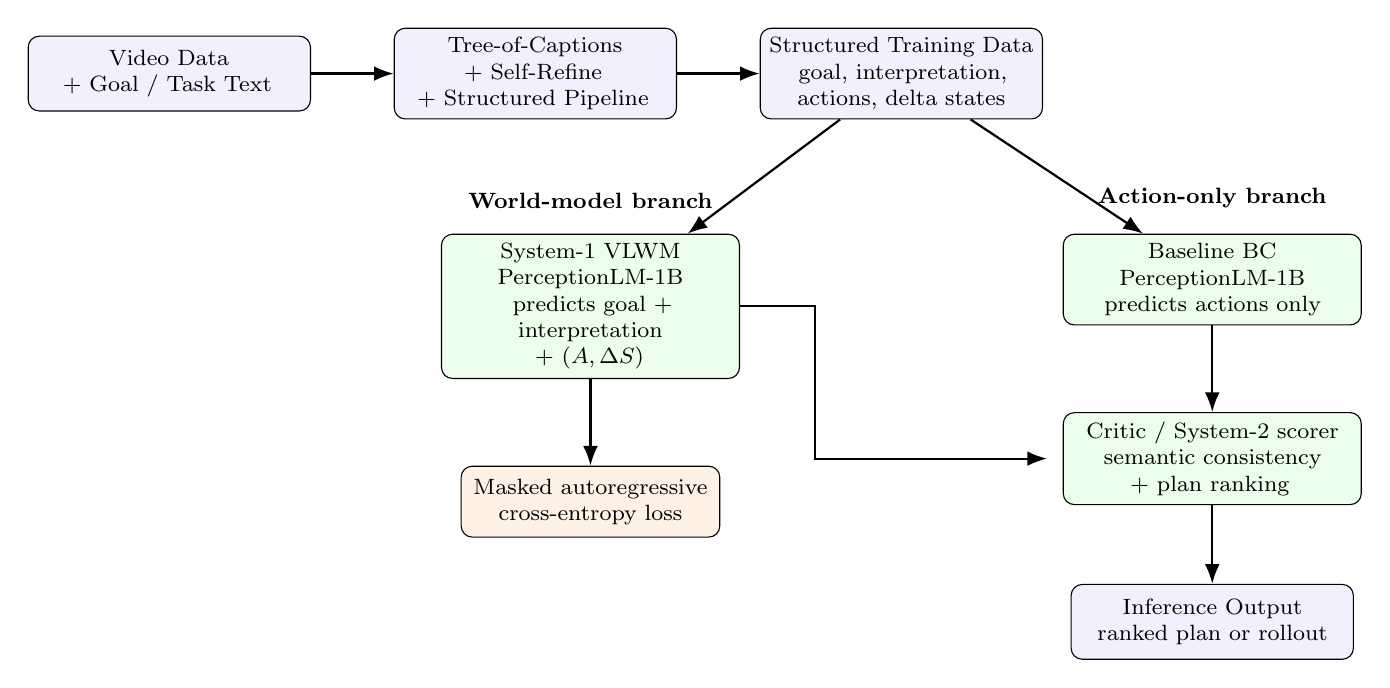
\begin{tikzpicture}[
    node distance=1.0cm and 1.05cm,
    font=\footnotesize,
    box/.style={draw, rounded corners, align=center, text width=3.35cm, minimum height=0.95cm, fill=blue!6},
    branchbox/.style={draw, rounded corners, align=center, text width=3.55cm, minimum height=1.05cm, fill=green!8},
    lossbox/.style={draw, rounded corners, align=center, text width=3.05cm, minimum height=0.9cm, fill=orange!10},
    arrow/.style={-{Latex[length=2.5mm]}, thick}
]
\node[box] (video) {Video Data \\ + Goal / Task Text};
\node[box, right=of video] (toc) {Tree-of-Captions \\ + Self-Refine \\ + Structured Pipeline};
\node[box, right=of toc] (trainset) {Structured Training Data \\ goal, interpretation, \\ actions, delta states};

\node[branchbox, below left=1.45cm and 0.25cm of trainset] (system1) {System-1 VLWM \\ PerceptionLM-1B \\ predicts goal + interpretation \\ + $(A,\Delta S)$};
\node[branchbox, below right=1.45cm and 0.25cm of trainset] (baseline) {Baseline BC \\ PerceptionLM-1B \\ predicts actions only};

\node[lossbox, below=1.1cm of system1] (celoss) {Masked autoregressive \\ cross-entropy loss};
\node[branchbox, below=1.1cm of baseline] (critic) {Critic / System-2 scorer \\ semantic consistency \\ + plan ranking};

\node[box, below=of critic] (output) {Inference Output \\ ranked plan or rollout};

\draw[arrow] (video) -- (toc);
\draw[arrow] (toc) -- (trainset);
\draw[arrow] (trainset) -- (system1);
\draw[arrow] (trainset) -- (baseline);
\draw[arrow] (system1) -- (celoss);
\draw[arrow] (baseline) -- (critic);
\draw[arrow] (system1.east) -- ++(0.95,0) |- ([xshift=-2mm]critic.west);
\draw[arrow] (critic) -- (output);

\node[align=center, above=0.2cm of system1, font=\footnotesize\bfseries] {World-model branch};
\node[align=center, above=0.2cm of baseline, font=\footnotesize\bfseries] {Action-only branch};
\end{tikzpicture}
}
\caption{Architecture overview of the project pipeline. Video observations and task goals are converted into structured supervision, then used to compare a System-1 world-model branch against an action-only baseline. A critic reranks candidate plans at inference time.}
\label{fig:architecture}
\end{figure}

Table~\ref{tab:datasets} summarizes the primary datasets emphasized in the current project narrative, and Table~\ref{tab:hyperparams} lists the key training settings.

\begin{table}[t]
\centering
\caption{Primary procedural video datasets used in the project discussion and experiments.}
\label{tab:datasets}
\begin{tabular}{ll}
\toprule
Dataset & Role in the project \\
\midrule
COIN & instructional task steps and temporal structure \\
CrossTask & cross-task procedural supervision and split-based evaluation \\
\bottomrule
\end{tabular}
\end{table}

\begin{table}[t]
\centering
\caption{Key training hyperparameters extracted from the project configuration files.}
\label{tab:hyperparams}
\begin{tabular}{lll}
\toprule
Setting & System-1 & Baseline \\
\midrule
Backbone & \texttt{perceptionlm-1b} & \texttt{perceptionlm-1b} \\
Objective & next-token CE & next-token CE \\
Target & goal + interpretation + $(A,\Delta S)$ & actions only \\
Batch size & 128 & 128 \\
Epochs & 1 & 1 \\
Learning rate & $2\times10^{-5}$ & $2\times10^{-5}$ \\
Weight decay & 0.01 & 0.01 \\
Scheduler & cosine, 3\% warmup & cosine, 3\% warmup \\
Context limit & 11{,}500 & 4{,}096 \\
\bottomrule
\end{tabular}
\end{table}

\section{Experiments and Results}
\subsection{Experimental Design}
The experimental goal is to measure whether explicit state-change supervision improves procedural planning quality relative to an action-only baseline. The branch structure of the repository suggests a two-level evaluation story. First, the paper-aligned \texttt{vlwm\_planning} setup compares matched System-1 and baseline decoders using unified JSONL training files and aligned CrossTask/COIN-style splits. Second, the richer \texttt{TreeOfCaption} and \texttt{JEPA\_Latent\_Generation} branches extend this into a broader planning stack with goal prediction, critic scoring, latent bridges, retrieval evaluation, and robustness analysis. For the report, this means the core comparison should remain the System-1 versus baseline experiment, while the branch-specific modules can be presented as the wider project context and future-ready extensions.

At minimum, the final evaluation should report:
\begin{itemize}
  \item token-level validation loss for both models;
  \item sequence-level action prediction quality on held-out tasks;
  \item state-change prediction quality for the System-1 model;
  \item qualitative examples showing whether predicted delta states make the generated plan easier to interpret.
\end{itemize}

\subsection{Evaluation Protocol}
The evaluation plan follows the same layered structure as the implementation. In the paper-aligned \texttt{vlwm\_planning} branch, the primary comparison is between the System-1 model and the action-only baseline on matched held-out splits from CrossTask and COIN. This comparison should report validation loss together with task-level action quality so that the two models are compared under the same backbone, optimizer, and data regime. For the System-1 model, evaluation should also inspect whether predicted delta states remain coherent with the intended task and whether they make the generated rollout easier to interpret.

The broader repository branches define how this evaluation can be extended beyond simple loss reporting. The \texttt{TreeOfCaption} branch contains end-to-end evaluation and inference scripts that support rollout generation, critic data preparation, and full evaluation passes over structured planning outputs. The \texttt{JEPA\_Latent\_Generation} branch adds complementary metrics through V-JEPA-grounded evaluation scripts for consistency retrieval, robustness testing, critic-based scoring, and ablation studies. In practice, this means the final paper can report a compact main result table for the System-1 versus baseline comparison, while also adding a smaller set of supporting results on reranking quality, retrieval-style semantic consistency, and robustness under branch-specific ablations.

\subsection{Results}
Table~\ref{tab:results} is structured around the core comparison of the project: whether adding goal interpretation and delta-state supervision improves procedural prediction relative to an action-only baseline. The final table should report the matched validation loss for both models, the main action-quality metric on held-out tasks, and the state-quality metric for the System-1 model. Together, these values will show whether the richer target structure improves planning-oriented behavior rather than only next-token fitting.

In addition to the main table, the final analysis should include a small number of qualitative examples. These examples should compare generated action sequences and intermediate state predictions on the same task instance so that the paper can show not only whether System-1 performs better numerically, but also whether its outputs are easier to interpret and more consistent with the intended goal.

\begin{table}[t]
\centering
\caption{Quantitative comparison between the action-only baseline and the System-1 model. Final metrics should be inserted from the completed evaluation runs.}
\label{tab:results}
\begin{tabular}{lcccc}
\toprule
Model & Val Loss $\downarrow$ & Action Score $\uparrow$ & State Score $\uparrow$ & Notes \\
\midrule
Baseline & \fillme{xx.xx} & \fillme{xx.x} & -- & action-only decoding \\
System-1 & \fillme{xx.xx} & \fillme{xx.x} & \fillme{xx.x} & goal + state supervision \\
\bottomrule
\end{tabular}
\end{table}

\section{Discussion}
This project highlights a practical tension in multimodal planning research. On one hand, language modeling offers a simple and scalable way to train over mixed video-text corpora. On the other hand, planning requires more than next-step imitation; it requires some representation of what changes in the world when an action is taken. The System-1 formulation addresses this by turning state transitions into explicit language targets.

One strength of the current design is experimental control. The baseline and System-1 pipelines differ mainly in the structure of the supervision target, not in unrelated training machinery. That makes the study easier to interpret. Another strength is reproducibility: the pipeline is transparent, configuration-driven, and already organized around separate schema builders, conditioning modules, and a shared trainer runtime.

There are also limitations. First, serialized visual context is only as informative as the upstream extraction process, which is abstracted away in the current training code. Second, the quality of state-change supervision depends on how consistently the intermediate annotations are produced across tasks and datasets. Third, delta-state descriptions may vary in granularity across datasets, which could affect cross-dataset consistency.

Future work should extend the project in three directions. The first is evaluation, especially task-level success measures and structured state consistency metrics. The second is richer multimodal grounding, such as tighter alignment between frame-level evidence and textual state changes. The third is planning-time use: rather than treating generated states only as supervision targets, the model could use them as internal rollouts for action selection or self-correction.

\section{Conclusion}
We presented a research-oriented training framework for procedural planning with a vision-language world model. The central idea is to move beyond action-only decoding and explicitly supervise goal interpretation together with action-conditioned state changes. The resulting System-1 formulation remains simple to train because it uses the same autoregressive cross-entropy objective as a standard causal language model, but it offers a more structured target that is better aligned with planning. The project therefore contributes both a concrete training formulation and a modular implementation pipeline for testing whether explicit world-state reasoning improves procedural video understanding.

\bibliographystyle{plainnat}
\bibliography{references}

\clearpage
\appendix
\section{Appendix: Individual Contributions}
This appendix is required for fair assessment and should be completed with precise team-level details before submission. The categories below are intentionally aligned with the course guidelines.

\subsection{Problem Formulation}
\textbf{\fillme{Member name}} contributed to identifying the research question, defining the comparison between action-only imitation and state-aware planning, and reviewing the core papers on world models and procedural video understanding.

\subsection{Model Development}
\textbf{\fillme{Member name}} implemented the training code, including the data schema, conditioning pipeline, loss masking, trainer runtime, and configuration files. \textbf{\fillme{Member name}} contributed to prompt formatting, input serialization, and debugging training scripts.

\subsection{Experiments and Evaluation}
\textbf{\fillme{Member name}} prepared dataset splits, validated JSONL formats, and launched the System-1 experiments. \textbf{\fillme{Member name}} handled the baseline experiments, metric collection, and comparison tables. \textbf{\fillme{Member name}} analyzed failure cases and selected qualitative examples.

\subsection{Writing the Paper}
\textbf{\fillme{Member name}} drafted the introduction and related work. \textbf{\fillme{Member name}} wrote the methodology section and described the implementation. \textbf{\fillme{Member name}} prepared the experiments, discussion, and conclusion sections. \textbf{\fillme{Member name}} acted as lead editor to unify tone, structure, and formatting.

\subsection{Collaboration and Discussion}
\textbf{\fillme{Member name}} coordinated team meetings, tracked milestones, and consolidated mentor feedback. \textbf{\fillme{Member name}} maintained the shared repository and ensured the paper and code remained synchronized.

\subsection{Additional Contributions}
Add any contributions here that do not fit neatly into the categories above, such as literature curation, slide preparation, figure design, or reproducibility checks.

\end{document}
